\documentclass[12pt,a4paper]{report}
\usepackage[T1]{fontenc}
\usepackage[utf8]{inputenc}
\usepackage{charter}
\usepackage{ngerman}
\usepackage[left=2cm,right=2cm,top=2cm,bottom=2cm]{geometry}
\usepackage{amsmath}
\usepackage{pgfplots}
\usepackage{tikz}
\usepackage{tcolorbox}
\tcbuselibrary{skins,breakable}
\usetikzlibrary{shadings,shadows}
\usepackage{graphicx}

\newenvironment{gblock}[1]{
    \tcolorbox[beamer,
        noparskip,
        colback=green!50!,
        colbacklower=green!75!green,
        title=#1]}
{\endtcolorbox}

\newcommand{\cas}[1]{\textbf{CAS-Eingabe: }\ \ \texttt{#1}}


\begin{document}
	\noindent
	\Large
	Ganzrationale Funktionen
	\large
	\\
	\begin{gblock}{Übersicht}
		Eine ganzrationale Funktion ist eine Summe aus mehreren Potenzfunktionen, die mit natürlichen Exponenten beschrieben werden können.
		\paragraph{Beispiel:} \mbox{}
		\begin{align*}
			f(x) = 3x^4 - 4x^2
		\end{align*}
		\begin{center}
			\begin{tikzpicture}
				\begin{axis}[
					axis lines = middle,
					xlabel = $x$,
					ylabel = $f(x)$,
				]
				\addplot[domain=-1.5:1.5, samples=100, color=red]{3*x^4-4*x^2};
				\end{axis}
			\end{tikzpicture}
		\end{center}
		\cas{f(x):=$3x^4 - 4x^2$}
	\end{gblock}
	
	\begin{gblock}{Eigenschaften}
	Ganzrationale Funktionen haben verschiedene Eigenschaften, die von den Potenzen der Funktion abhängen.
	\paragraph{Grad:} Der Grad einer ganzrationalen Funktion ist der höchste Exponent, mit dem die Variable x vorkommt. Er bestimmt das Verhalten der Funktion gegen $+\infty$ und $-\infty$. (Randverhalten)
	\paragraph{Nullstellen:} Die Nullstellen einer Funktion sind die x-Werte, für die die Funktion den Wert Null annimmt.
	\paragraph{Graph:} Der Graph einer ganzrationalen Funktion ist immer eine glatte Kurve ohne Ecken oder Spitzen.
	\paragraph{Verhalten nahe Null:} Der Graph einer Funktion $f(x)$ verhält sich nahe Null wie der Graph der Funktion $g(x)$ mit $g(x)$ als der Summand mit dem kleinsten Exponenten von $x$ addiert mit dem Summanden ohne $x$
\end{gblock}
	\newpage
	\noindent
	\Large Beispielhafte Funktionsanalyse
	\large
	\begin{gblock}{Symmetrie}
		Die Symmetrie der Funktion kann mit folgendem Ansatz bestimmt werden:
		\begin{align*}
			f(-x) &= f(x) \to \text{Achsensymmetrisch} \\
			f(-x) &= -f(x) \to \text{Punktsymmetrisch}
		\end{align*}
		Sollte keiner der beiden Ansätze funktionieren, liegt keine Symmetrie vor.
		\begin{align*}
			f(x) &= 3x^4 - 4x^2 \\
			f(-x) &= 3x^4 - 4x^2 \\
		\end{align*}
		Es liegen ausschließlich gerade Exponenten vor, weswegen diese Bedingung erfüllt ist: Die Funktion ist Achsensymmetrisch.
		\\
		\cas{f(x):=$3x^4-4x^2$} \\
		\cas{f(x)=f(-x) \ \ \ \ \ \ \ \ \ \ \ \ \ \ \ true}
	\end{gblock}
	\begin{gblock}{Nullstellen}
		Für die Nullstellen wird der folgende Ansatz gewählt:
		\begin{align*}
			f(x) &= 0 \\
			3x^4 - 4x^2 &= 0 \\
			x^2 &\cdot (3x^2 - 4) \\
			\Rightarrow x_1 &= 0\ \text{(Satz vom Nullprodukt)} \\
			3x^2 - 4 &= 0\ \Bigl| +4 \\
			3x^2 &= 4\ \Bigl|\div 3 \\
			x^2 &= \frac{4}{3}\ \Bigl|\sqrt{} \\
			x_2 &= \frac{2}{\sqrt{3}}\ \land x_3 = \frac{-2}{\sqrt{3}}
		\end{align*}
		Für die Berechnung im Computer Algebra System (CAS) wird folgender Befehl verwendet: \\
		\cas{f(x):=$3x^4$ - $4x^2$} \\
		\cas{solve(f(x)=0,x)}
	\end{gblock}
	\begin{gblock}{Ableitungen und Stammfunktion}
		\begin{align*}
			f'(x) &= 12x^3 -8x \\
			f''(x) &= 36x^2 - 8 \\
			f'''(x) &= 72x \\
			F(x) &= \frac{3}{5}x^5 - \frac{4}{3}x^3
		\end{align*}
		Allgemeine Form:
		\begin{align*}
			f(x) &= ax^b \\
			f'(x) &= a \cdot b \cdot x^{b-1} \\
			F(x) &= \frac{a}{b}\cdot x^{b+1}
		\end{align*}
		\cas{$\frac{d}{dx}(f(x))$   (Ableitung)} \\
		\cas{$\int f(x) dx$   (Stammfunktion)}
	\end{gblock}
	\begin{gblock}{Extremstellen}
		Für die Extremstellen einer Funktion wird sowohl die notwendige, als auch die hinreichende Bedingung benötigt:
		\begin{align*}
			\texttt{notwendige Bedingung für EST:}& f'(x) = 0 \\
			12x^3 - 8x &= 0 \\
			x \cdot (12x^2 - 8) &= 0 \\
			\texttt{Satz vom Nullprodukt}: x_1 &= 0 \\
			12x^2 - 8 &= 0\ \Bigl|+8\\
			12x^2 &= 8\ \Bigl|\div 12\\
			x^2 &= \frac{8}{12} \\
			x^2 &= \frac{2}{3}\ \Bigl|\sqrt{} \\
			x_2 = \sqrt{\frac{2}{3}} &\land x_3 = -\sqrt{\frac{2}{3}} \\
			\texttt{hinreichende Bedingung für EST:}& f'(x) = 0 \land f''(x) \ne 0 \\
			f''(0) &= 36 \cdot 0^2 - 8 = -8 < 0 \to HP \\
			f''(\sqrt{\frac{2}{3}}) &= 36 \cdot (\sqrt{\frac{2}{3}})^2 - 8 \\
			\Leftrightarrow f''(\sqrt{\frac{2}{3}}) &=36\cdot \frac{2}{3} - 8 \\
			\Leftrightarrow f''(\sqrt{\frac{2}{3}}) &= 16-8 = 8 > 0 \to TP \\
			f''(-\sqrt{\frac{2}{3}}) &= 36 \cdot (-\sqrt{\frac{2}{3}})^2 - 8 \\
			\Rightarrow f''(-\sqrt{\frac{2}{3}}) &= 8 > 0 \to TP
		\end{align*}
	\end{gblock}
	
	\begin{gblock}{Wendestellen}
		Für die Wendestellen wird sowohl die notwendige, als auch die hinreichende Bedingung benötigt:
		\begin{align*}
			\texttt{notwendige Bedingung für WDS}&: f''(x) = 0 \\
			36x^2 - 8 &= 0\ \Bigl|+8 \\
			36x^2 &= 8\ \Bigl|\div 36\\
			x^2 &= \frac{8}{36}\\
			x^2 &= \frac{2}{9}\ \Bigl|\sqrt{} \\
			x_1 = \sqrt{\frac{2}{9}} &\land x_2 = -\sqrt{\frac{2}{9}} \\
			\texttt{hinreichende Bedingung für WDS}&: f''(x) = 0 \land f'''(x) \ne 0 \\
			f'''(\sqrt{\frac{2}{9}}) &= 72 \cdot \sqrt{\frac{2}{9}} \ne 0 \to WDS \\
			f'''(-\sqrt{\frac{2}{9}}) &= 72 \cdot \sqrt{\frac{2}{9}} \ne 0 \to WDS \\
		\end{align*}
	\end{gblock}
	
	\newpage
	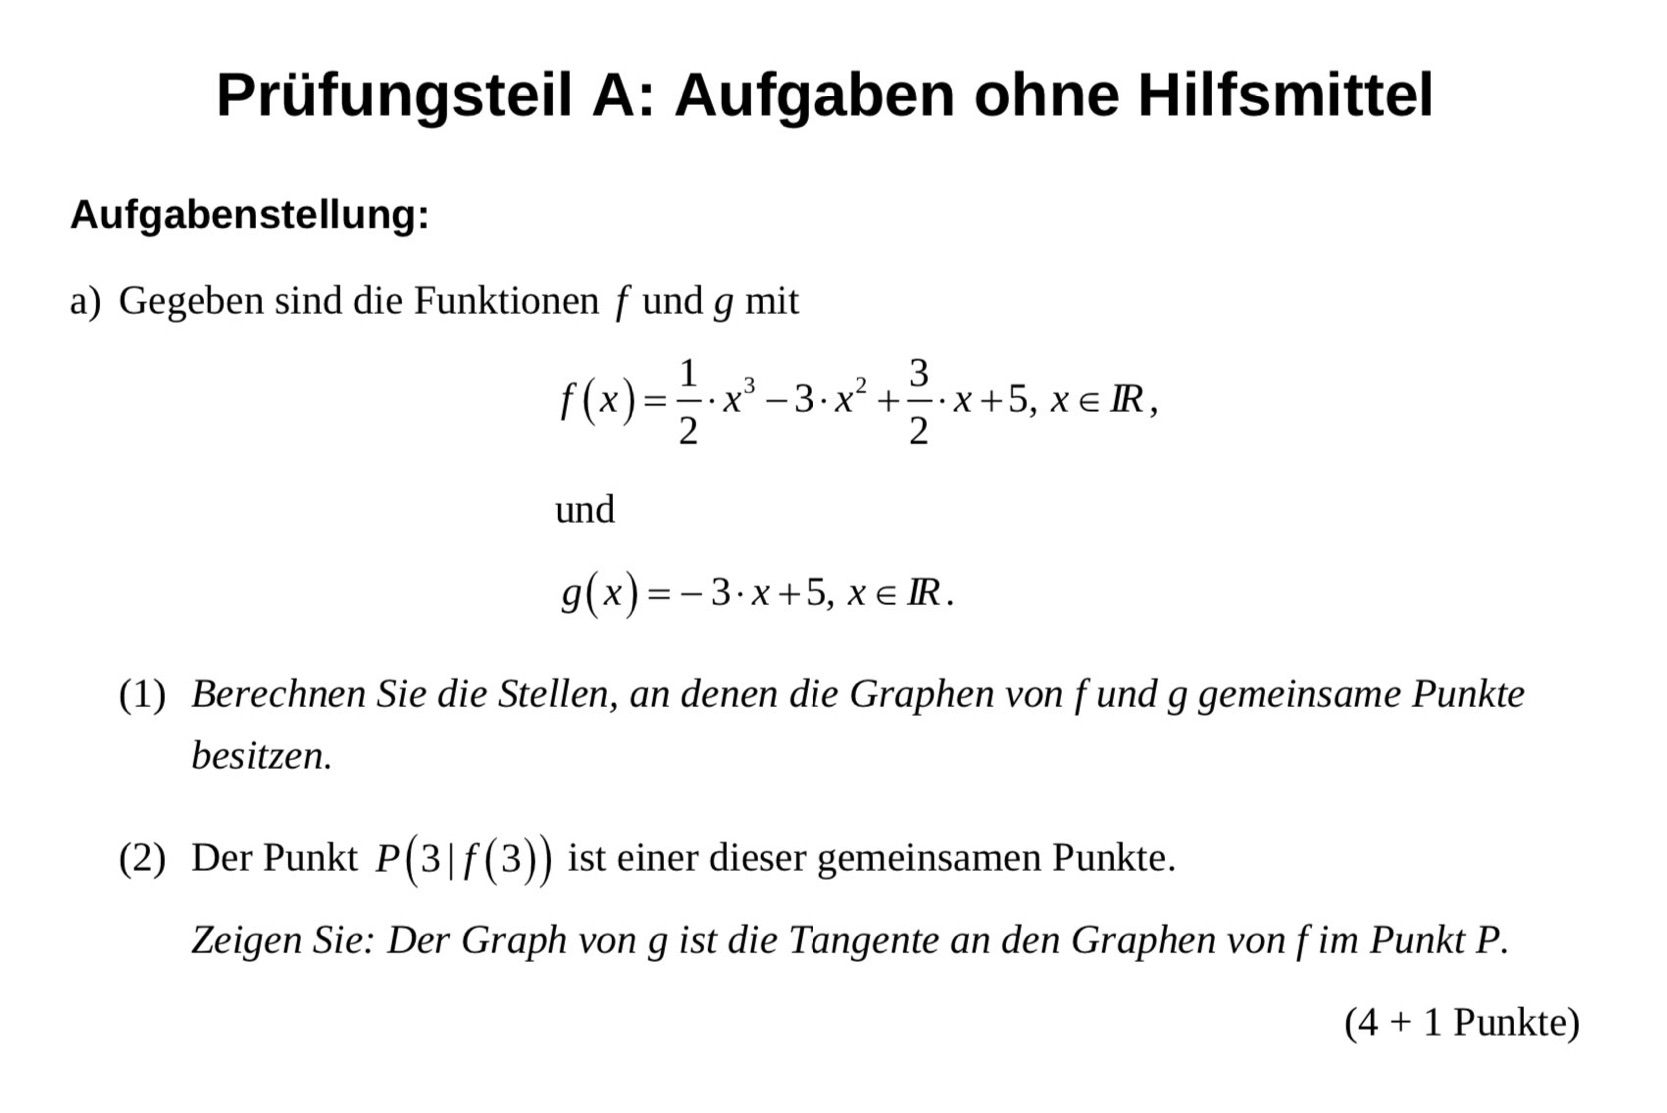
\includegraphics[width=\textwidth]{Abituraufgabe.JPG}
	\paragraph{a:1)}
	\begin{align*}
		f(x) &= g(x) \\
		\frac{1}{2}x^3 - 3x^2 + \frac{3}{2}x + 5 &= -3x+5\ \Bigl|-5 \\
		\frac{1}{2}x^3 - 3x^2 + \frac{3}{2}x &= -3x\ \Bigl|+3x \\
		\frac{1}{2}x^3 - 3x^2 + \frac{9}{2}x &= 0  \\
		x \cdot (\frac{1}{2}x^2 - 3x + \frac{9}{2}) &= 0 \\
		\texttt{Satz vom Nullprodukt}& \\
		\Rightarrow x_1 &= 0 \\
		\frac{1}{2}x^2 - 3x + \frac{9}{2} &= 0\ \Bigl|-\frac{9}{2} \\
		\frac{1}{2}x^2 - 3x &= -\frac{9}{2}\ \Bigl|\div \frac{1}{2} \\
		x^2 - 6x &= -\frac{18}{2} \\
		x^2 - 6x &= -9\ \Bigl|+9 \\
		x^2 - 6x + 9 &= 0 \\
		p.q.& \\
		x_{2} &= -\frac{p}{2} \pm \sqrt{(\frac{p}{2})^2 - q} \\
		x_{2} &= -\frac{-6}{2} \pm \sqrt{(\frac{-6}{2})^2 - 9} \\
		x_{2} &= 3 \pm \sqrt{-3^2 - 9} \\
		x_{2} &= 3
	\end{align*}
	\paragraph{a:2)}
	\begin{align*}
		f'(3) &= g'(3) \\
		f'(x) &= \frac{3}{2}x^2 - 6x + \frac{3}{2} \\
		g'(x) &= -3 \\
		f'(3) &= \frac{3}{2} \cdot 9 - 18 + \frac{3}{2} \\
		&= 13,5 - 18 + \frac{3}{2} \\
		&= -4,5 + 1,5 \\
		&= -3 \\
	\end{align*}
	Da die Steigung von $g$ und $f$ im Punkt $P$ identisch ist, ist $g$ die Tangente von $f$ im Punkt $P$
\end{document}